\chapter{GÉNÉRALITÉ SUR LE MACHINE LEARNING}
\begin{spacing}{1.2}
\minitoc
\thispagestyle{MyStyle}
\end{spacing}
\newpage

Le machine learning, abrégé ML, représente l’une des branches les plus captivantes de l’intelligence artificielle, un sujet qui pourrait remplir un livre entier à lui seul. Cette approche technologique révolutionnaire permet aux experts en données, communément appelés « Data Scientists », d’alimenter les algorithmes avec des ensembles de données, donnant ainsi aux machines la capacité d’apprendre et de prendre des décisions sans nécessiter de programmation informatique préalable.
\\
Dans ce chapitre, nous commencerons par une présentation du machine learning (ML), nous aborderons ensuite la classification des méthodes et les algorithmes de ML, et nous découvrirons enfin à travers ce chapitre les étapes du processus du ML.

\section{Présentation de machine leaning}

\subsection{Contexte}
Nous générons toujours plus de données chaque jour avec la multiplicité des technologies que nous utilisons 
(smartphones, ordinateurs, tablettes, objets connectés…). Tous ces appareils génèrent une quantité de données massive. Une personne génère en moyenne 1,7 Mo de 
données par seconde en 2020. L’ensemble de ces données est stocké en bases numériques et représente une source d’informations considérable : c’est le Big Data \cite{Azencott_chloe}. 
Mais sans traitement adéquat ni stratégie d’analyse efficace, cette masse de données ne resterait qu’un amas d’octets problématiques à entasser. C’est à ce moment 
que le Machine Learning intervient et permet de tirer profit de ces données.

\subsection{Définition}
L'apprentissage automatique, un sous-ensemble de l'intelligence artificielle, donne aux ordinateurs la capacité d'apprendre et de faire des prédictions ou des décisions basées sur des données. Cela implique le développement d’algorithmes capables d’apprendre et de s’améliorer automatiquement à partir de l’expérience sans être explicitement programmés. 

\subsection{Rôle de machine learning dans l'intelligence artificielle}
Le machine learning est crucial pour IA car il permet aux systèmes d'apprendre et de s'améliorer à partir de données, sans intervention humaine. Cette capacité d'adaptation rend les systèmes d'IA plus précis et efficaces, en particulier dans des tâches complexes comme la reconnaissance d'images et la compréhension du langage naturel. De plus, le machine learning est au cœur de nombreuses applications pratiques, de la recommandation de produits à la détection de fraudes. Il permet également l'automatisation de tâches, réduisant les coûts et augmentant l'efficacité. En constante évolution, le machine learning favorise l'innovation continue et la personnalisation des expériences utilisateur, transformant ainsi divers secteurs et améliorant la qualité de nombreux services.

\section{Fonctionnement de machine learning}
Le ML fonctionne en suivant un processus général composé de quatre étapes principales : la collecte de données, le prétraitement des données, la formation du modèle et l'évaluation du modèle \cite{fastercapital_ml}.

\subsection{Collecte de données}
La collecte de données est la première et la plus importante étape de l'apprentissage automatique, où les données pertinentes et suffisantes sont collectées à partir de diverses sources, telles que des bases de données, des pages Web, des capteurs, des enquêtes, etc. La qualité et la quantité des données déterminent les performances et la précision du modèle d'apprentissage automatique. Il est donc essentiel de collecter des données représentatives, diverses et impartiales.

\subsection{Prétraitement des données}
Le prétraitement des données est la deuxième étape du ML, où les données brutes sont nettoyées, transformées et préparées pour le modèle. Le prétraitement des données implique des tâches telles que la gestion des valeurs manquantes, des valeurs aberrantes et du bruit, le codage des variables catégorielles, la mise en échelle des variables numériques, l'ingénierie des fonctionnalités, la sélection des fonctionnalités et le fractionnement des données.\\ 
Le prétraitement des données vise à améliorer la qualité et la convivialité des données et à réduire la complexité et la dimensionnalité des données.

\subsection{Entraînement de modèle}
L'entraînement de modèle est la troisième étape du ML, où le modèle est construit et formé sur les données pré-traitées. Il implique de choisir un algorithme d'apprentissage automatique approprié, tel qu'un arbre de décision, un réseau de neurones, une machine à vecteurs de support, etc., et d'ajuster ses paramètres, tels que le taux d'apprentissage, le nombre d'itérations, le terme de régularisation, etc.\\ 
L'entraînement sur modèle vise à trouver les paramètres optimaux qui minimisent la fonction d’erreur ou de perte et maximisent la précision ou la mesure de performance.

\subsection{Évaluation du modèle}
L'évaluation du modèle est la quatrième et dernière étape du ML, où le modèle est testé et validé sur des données invisibles. L'évaluation du modèle consiste à mesurer la capacité de généralisation et la robustesse du modèle d'apprentissage automatique, à l'aide de mesures telles que l'exactitude, la précision, le rappel, le score f1, la courbe d'évaluation, etc. \\ 
Elle vise à évaluer l'efficacité et la fiabilité du modèle d'apprentissage automatique et à identifier les domaines d'amélioration ou de modification.
\begin{figure}[H]%
    \center%
    \setlength{\fboxsep}{5pt}%
    \setlength{\fboxrule}{0.5pt}%
    \fbox{
    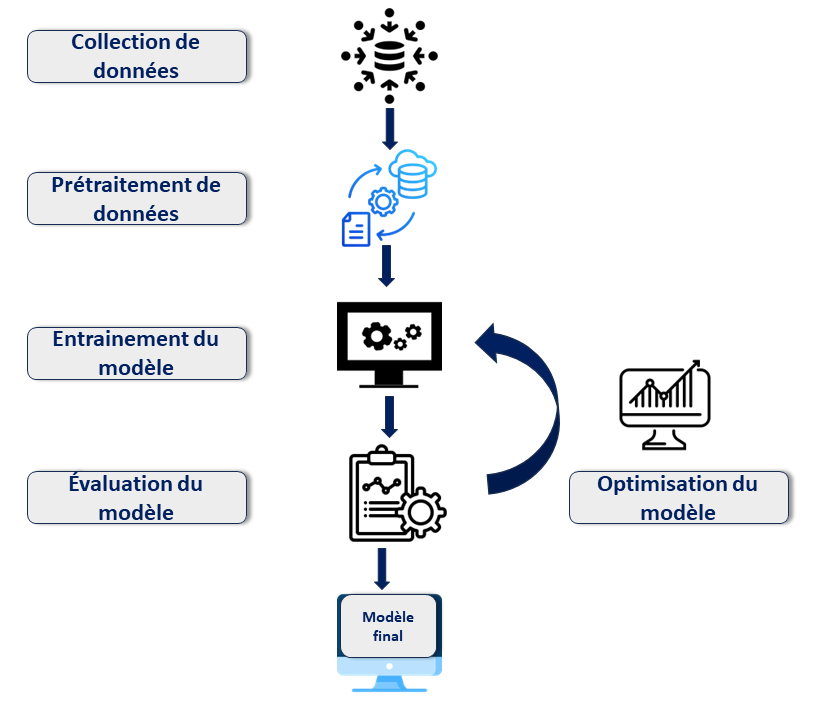
\includegraphics[width=10cm,height=6cm]{images/fonctionnement de ml.png}%
    }
    \caption{Fonctionnement de ML.}%
\end{figure}

\section{Classification des approches de machine learning et leurs algorithmes}

Les approches et algorithmes d'apprentissage automatique sont les moteurs des progrès de l'intelligence artificielle et de l'analyse des données. Ces approches et algorithmes permettent aux machines d'apprendre des données et de faire des prédictions ou des décisions sans programmation explicite. En analysant de grands ensembles de données et en identifiant les modèles, les algorithmes d'apprentissage automatique peuvent découvrir des informations cachées et fournir des prédictions précieuses pour diverses industries et applications.

Il existe plusieurs types d'approches et d'algorithmes d'apprentissage automatique, chacun conçu pour résoudre différents types de problèmes. Dans cette partie, nous allons explorer certaines des principales approches et algorithmes les plus couramment utilisés et leurs applications.

\subsection{Apprentissage supervisé}
L'apprentissage supervisé consiste à entraîner des modèles sur des ensembles de données étiquetés, où chaque point de données est associé à une valeur de résultat ou de cible connue \cite{mohri2012}. Ces modèles apprennent à partir de ces données étiquetées et sont capables de faire des prédictions sur des données inconnues ou futures. 
\begin{figure}[H]%
    \center%
    \setlength{\fboxsep}{5pt}%
    \setlength{\fboxrule}{0.5pt}%
    \fbox{
    \includegraphics[width=10cm,height=6cm]{images/apprentissage supervisé.png}%
    }
    \caption{Apprentissage supervisé.}%
\end{figure}
Fondamentalement, le ML supervisé revient à apprendre à une machine à construire une fonction \( f \) telle que \( Y = f(X) \), \( Y \) étant un ou plusieurs résultats d'intérêt calculés en fonction des données d'entrée \( X \) effectivement à la disposition de l'utilisateur. \( Y \) peut être une grandeur continue (une température par exemple), et on parle alors de régression, ou discrète (une classe, chien ou chat par exemple), et on parle alors de classification. L'apprentissage supervisé est donc divisé en deux catégories principales : la classification et la régression.

\subsubsection{Les algorithmes de classification}
La classification automatique, également connue sous le nom de classification supervisée, est une méthode algorithmique qui consiste à attribuer des classes ou des catégories discrètes à des objets en fonction de caractéristiques ou de variables d'entrée. L'objectif est de construire un modèle qui puisse prédire la classe correcte pour de nouveaux exemples basés sur des exemples préalablement étiquetés dans l'ensemble de données d'apprentissage. Les algorithmes de classification sont largement utilisés dans divers domaines tels que la reconnaissance de texte, la détection de spam, la classification d'images et bien d'autres.

Différents algorithmes de classification existent, chacun avec ses propres caractéristiques et fonctionnalités. Certains des algorithmes de classification les plus couramment utilisés comprennent : \textbf{Arbres de décision}, \textbf{Machine à Vecteur de support (SVM)}, \textbf{K plus proches voisins (KNN)}, \textbf{Réseaux de neurones artificiels}, etc.

\subsubsection{Les algorithmes de régression}
Contrairement à la classification qui prédit une catégorie ou une étiquette, les modèles de régression prédisent une valeur de sortie continue, en fonction de la variable indépendante d’entrée. Cette technique est utilisée lorsque la variable de sortie à prédire doit être une valeur continue, soit par exemple pour les prédictions météorologiques ou pour les tendances de marché. Différents modèles de régression existent et diffèrent dépendant de la relation entre la variable dépendante et indépendante considérée, ainsi que du nombre de variables indépendantes utilisées pour le modèle. Parmi les principaux modèles de régression : \textbf{Régression logistique binaire}, \textbf{Régression logistique multiclasse}, \textbf{Régression linéaire simple}, \textbf{Régression linéaire multiple}, \textbf{Régression à vecteurs de support (RVM)}, etc.

\subsection{Apprentissage non supervisé}
L'apprentissage non supervisé est un sous-champ d'apprentissage automatique qui se concentre sur l'identification des modèles et des relations cachés dans les données sans utiliser d'exemples étiquetés ou pré-classifiés \cite{sublime2022}. Contrairement à l'apprentissage supervisé, qui consiste à former un modèle sur un ensemble de données étiqueté et à l'utiliser pour faire des prédictions sur de nouvelles données invisibles, des algorithmes d'apprentissage non supervisés fonctionnent sur des données brutes et non marquées et visent à découvrir les structures ou les relations sous-adjacentes. L'algorithme doit découvrir par lui-même la structure plus ou moins cachée des données.
\begin{figure}[H]%
    \center%
    \setlength{\fboxsep}{5pt}%
    \setlength{\fboxrule}{0.5pt}%
    \fbox{
    \includegraphics[width=12cm,height=6cm]{images/apprentissage non-supervisé.png}%
    }
    \caption{Apprentissage non supervisés.}%
\end{figure}

Fondamentalement, le machine learning non supervisé revient à apprendre à une machine à construire une fonction \( f \) telle que \( Y = f(X) \), \( Y \) étant un ou plusieurs résultats d'intérêt calculés en fonction des données d'entrée \( X \) effectivement à la disposition de l'utilisateur. \( Y \) peut être une grandeur continue (par exemple, une caractéristique mesurée), et on parle alors de réduction de dimensionnalité ou de clustering, ou discrète (par exemple, un groupe ou une catégorie), et on parle alors de segmentation ou de classification automatique. L'apprentissage non supervisé est donc un processus visant à découvrir des structures ou des groupes naturels dans les données, sans qu'il soit nécessaire de fournir des exemples étiquetés.

\subsubsection{Les algorithmes de partitionnement ou le Clustering}
Les algorithmes de partitionnement sont des techniques d'apprentissage non supervisé qui visent à diviser un ensemble de données en plusieurs clusters ou groupes, où chaque cluster est une collection de points de données similaires. L'objectif est de partitionner les données de manière à ce que les points à l'intérieur de chaque cluster soient similaires les uns aux autres, tandis que les points de différents clusters soient différents. Parmi ceux-ci figurent: \textbf{k-means}, \textbf{Clustering hiérarchique}, \textbf{Mean Shift}, \textbf{DBSCAN}, etc.

\subsubsection{Les algorithmes de la réduction de la dimensionnalité}
La réduction de la dimensionnalité vise à réduire le nombre de variables aléatoires dans un ensemble de données, tout en préservant autant que possible les caractéristiques importantes des données. Cela est souvent nécessaire lorsque les données sont très complexes et comprennent un grand nombre de dimensions, ce qui peut rendre l'analyse et la visualisation difficiles. Il est couramment utilisé dans l'étape de pré-traitement des données, et il existe différents algorithmes de réduction de la dimensionnalité qui peuvent être utilisés, à savoir : \textbf{Auto-encodeurs}, \textbf{Décomposition en valeurs singulières (DVS)}, \textbf{Principal Component Analysis}, \textbf{Locally Linear}, etc.

\subsection{Apprentissage par renforcement}
L'apprentissage par renforcement ou le Reinforcement Learning (RL) en anglais est un sous-ensemble de l'apprentissage automatique qui permet à un système piloté par l'IA (parfois appelé un agent) d'apprendre par tâtonnements à l'aide d'un retour d'information à partir de ses actions. Cette rétroaction est soit négative soit positive, qualifiée de punition ou de récompense avec, bien sûr, l'objectif de maximiser la fonction de récompense. RL apprend de ses erreurs et offre une intelligence artificielle qui imite l'intelligence naturelle aussi étroitement que possible.

En termes de méthodes d'apprentissage, RL est similaire à l'apprentissage supervisé uniquement en ce qu'il utilise la cartographie entre l'entrée et la sortie, mais c'est la seule chose qu'ils ont en commun. Alors que dans l'apprentissage supervisé, le retour d'information contient l'ensemble correct d'actions à prendre par l'agent. Dans le RL, il n'existe pas de clé de réponse de ce type. L'agent décide de ce qu'il faut faire lui-même pour effectuer la tâche correctement. Comparé à l'apprentissage non supervisé, le RL a des objectifs différents. L'objectif de l'apprentissage non supervisé est de trouver des similitudes ou des différences entre les points de données. L'objectif de RL est de trouver le modèle d'action le plus approprié pour maximiser la récompense cumulée totale pour l'agent RL. En l'absence d'ensemble de données de formation, le problème RL est résolu par les propres actions de l'agent avec l'apport de l'environnement.
De nombreux algorithmes d'apprentissage de renforcement utilisent des techniques de programmation dynamique \cite{vanotterlo2012}.
L'environnement dans un algorithme d'apprentissage de renforcement est généralement exprimé sous la forme d'un processus de décision de Markov (MDP), et presque tous les problèmes de RL sont formalisés à l'aide de MDP.\\
Dans l'apprentissage par renforcement, nous devons nous familiariser avec quelques concepts clés :
\begin{itemize}
	\item[\ding{118}] \textbf{L'agent} : qui est l'algorithme de ML (ou le système autonome).
	\item[\ding{118}] \textbf{L'environnement} : qui est l'espace adaptatif du problème avec des attributs tels que des variables, des valeurs limites, des règles et des actions valides.
	\item[\ding{118}] \textbf{L'action} : qui est une étape que l'agent de RL effectue pour naviguer dans l'environnement.
	\item[\ding{118}] \textbf{L'état} : qui est l'environnement à un moment donné.
	\item[\ding{118}] \textbf{La récompense} : qui est la valeur positive, négative ou nulle pour avoir effectué une action, en d'autres termes, la récompense ou la punition.
	\item[\ding{118}] \textbf{La politique} : qui est une stratégie que l'agent suit pour sélectionner une action dans chaque état.
	
\end{itemize}
\begin{figure}[H]%
    \center%
    \setlength{\fboxsep}{5pt}%
    \setlength{\fboxrule}{0.5pt}%
    \fbox{
    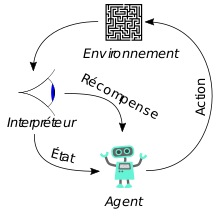
\includegraphics[width=8cm,height=6cm]{images/Reinforcement_learning_diagram_fr.svg.png}%
    }
    \caption{Apprentissage par renforcement.}%
\end{figure}
Dans le RL, de nombreux algorithmes sont utilisés tels que Q-Learning, Policy Gradient Methods, SARSA (State-Action-Reward-State-Action), Monte Carlo Methods, Temporal Difference Learning, etc. Tous ces algorithmes peuvent être regroupés en deux grandes catégories.
 
\subsubsection{Apprentissage par renforcement Axé sur un Modèle (Model-Based RL)}
Dans cette approche, l’agent construit un modèle interne de l’environnement. Ce modèle
peut être utilisé pour simuler les transitions d’états et les récompenses, ce qui permet à l’agent de
planifier ses actions avant de les exécuter dans l’environnement réel. Les algorithmes de RL axés
sur un modèle comprennent les méthodes de Monte Carlo avec modèle et certaines variantes
de l’apprentissage par différence temporelle. Parmi ces algorithmes figurent : \textbf{Model-Based
Actor-Critic}, \textbf{Dyna-Q}, \textbf{Dynammic Programming}, \textbf{Model Predictive Control} , etc.

\subsubsection{Apprentissage par renforcement sans Modèle (Model-Free RL)}
Dans cette approche, l'agent n'apprend pas explicitement un modèle de l'environnement, mais apprend plutôt à partir d'expériences directes dans l'environnement. L'agent utilise des interactions réelles avec l'environnement pour estimer la valeur des états ou des actions et pour apprendre une politique optimale sans avoir besoin de connaître les transitions d'états ou les récompenses à l'avance. Les algorithmes de RL sans modèle comprennent le Q-Learning, les méthodes de gradients de politique et certains types d'apprentissage par différence temporelle. ce sont: \textbf{Q-Learning}, \textbf{SARSA}, \textbf{Deep Q-Networks}, \textbf{Temporal Difference Learning} 

\section{Conclusion}
Ce deuxième chapitre a offert une introduction complète au machine learning, définissant
ses principes fondamentaux et soulignant son rôle central dans l’IA. Il a également décomposé
le processus du machine learning en étapes clés, de la collecte des données à l’évaluation des
modèles, tout en survolant les principales approches du machine learning, notamment l’apprentissage
supervisé, non supervisé et par renforcement, offrant ainsi un aperçu des algorithmes associés.